\chapter{Kata Containers in edge cloud environment}
\label{chapter:implementation}

\textcolor{red}{Come up with better chapter name}

Telco systems are a complex environment with multiple requirements for connectivity and performance. This chapter discusses the requirements of telco systems, implementation and possible limitations of Kata Containers in this environment. The performance and tests are described in Chapter \ref{chapter:evaluation}. The features discussed in this chapter are related to Kubernetes, the container orchestrator, configurations.

\section{CPU}

Telecommunication applications are computing heavy, which require efficient usage of resources. One of the requirements telco applications have for infrastructure is the support for core isolation. This feature allows dedicating a single core to a process in order to minimize interruptions for the process. Core isolation involves removing all user-space threads, unbound kernel threads and blocks interruptions from the system \cite{CPUisolation}. The benefit of a dedicated core for a process is enhanced performance and extended use of CPU caches.

The core isolation is accomplished with a specific Kubernetes plugin, such as Intel CMK\cite{IntelCMK} or Nokia CPU Pooler\cite{NokiaCPUPooler}. These plugins manage predefined physically separated pools of resources between applications. CPU Pooler supports two explicit types of CPU pools; exclusive and shared. Kubernetes allocates resources to a container on container creation. If the container has not requested specific resources from these pools, it will be assigned to a third, named default, pool. The exclusive pool allows applications for uninterrupted resources and is preferred for latency-sensitive workloads.

Kata Containers the architecture includes a Kata-agent and a guest kernel for each pod as described in Figure \ref{fig:KataContainersComponents}. These resources need to be assigned to a second core, a shared resource between other pods, or a core of the exclusive pool. The shared resources, defined by shared and default pool, can also host general cluster components such as monitoring and DNS.

\section{Memory}

Modern telco systems rely on high-throughput and low-latency data sharing between containers within pods. Writing and reading a shared block of memory between containers offers the fastest way for shared information. In Kubernetes, containers can share IPC namespaces inside a pod with the help of pod security policies \cite{PodSecurityPolicyKubernetes}. Configuration of these policies enables usage of HostIPC, which controls whether the pod containers can share host IPC namespace.

Kubernetes manages memory in blocks known as pages. In most systems, the default page size is 4 kilobytes; consequently, 1 megabyte of memory equals 256 pages. CPUs have a built-in memory management unit managing a list of these pages on hardware. This management unit, Translation Lookaside Buffer (TLB), has a fixed number of pages it can store. Once the number of pages exceeds the number defined in TLB, the system falls back to a slower, software-based address translation. This transition results in degraded performance. Since the number of pages TLB stores is fixed, the only way to decrease TLB miss is to increase the page size with huge pages. \cite{HugePagesOpenShift}

\subsection{Huge pages}

Huge pages is a memory page with a size larger than 4 kilobytes. In x86\_64 architectures, the two popular sizes are 2MB and 1GB. In order to use huge pages, the application must support the use the larger page sizes. The high-performance telco applications use huge pages; therefore, huge pages are crucial to maintaining performance.

Kubernetes supports the allocation and consumption of pre-allocated huge pages by applications in a pod \cite{HugePagesKubernetes}. Kata Containers also support using huge pages; however, it needs configuring explicitly in a custom Kata Containers kernel. As Kata Containers architecture consumes more memory than a native design with runC, the pod must be allocated enough resources to support huge pages.

\section{Storage}

High-performance Kubernetes storage options are usually limited to storage locating close to the computing unit. Thus, network storages or block storages hosted on a commercial cloud, which relies on data transmission via a network, are insufficient. Telco systems use three types of storage for high-performance applications: emptyDir, hostPath, and local. EmptyDir is a non-persistent volume, implying it does not retain data stored if the attached pod is removed from a node. In contrast, hostPath and local storages are Persistent Volumes (PV), a Storage Class type defined in Kubernetes. These storages are individuals of restructuring the cluster architecture and thus are applicable for storing user-related data or logs. In contrast, emptyDir is mainly used for session-specific data or offloading memory temporarily.

\subsection{emptyDir}

Kubernetes creates emptyDir volume during pod assignment to a node and lives as long as the pod runs on that node. emptyDir volume is initially empty. All containers in the pod of the emptyDir can read and write the files in the volume. Some use cases for emptyDir are scratch space during disk-based merge sort, checkpointing during a long computation in case of crashes, and holding files that a content-manager container fetches while a webserver container serves the data. \cite{VolumesKubernetes}

Various storage mediums such as disk or SSD can back emptyDir volumes. However, emptyDir also supports RAM-backed filesystem tmpfs, which offers a high-speed alternative to harddrive-based volumes. The system clears tmpfs filesystem on node reboot, and any data written on it counts against the container's memory limit. \cite{VolumesKubernetes}

\subsection{Persistent Volume}

Persistent Volume (PV) is a storage piece in the cluster, providing storage having a lifecycle independent of any individual pod using the PV. It is provisioned dynamically or by an administrator. Kubernetes supports filesystem and block-based persistent storage resources, such as Network Filesystem (NFS), SCSI over IP (iSCSI), local storage devices, or AWS Elastic Block Store \cite{AmazonEBS}.\cite{PV}

PVs can be mounted to nodes in Kubernetes with three different access modes: ReadWriteOnce, ReadOnlyMany, and ReadWriteMany. ReadWriteOnce allows only one node for read and write operations. ReadOnlyMany is a read-only mode allowing multiple nodes for simultaneous access. In contrast, ReadWriteMany allows multiple nodes for simultaneous read and write operations. Based on the type of PV, the support for access modes varies. In this Thesis, we will focus on two high-performing PV options, which are hostPath and local. \cite{PV} 

A hostPath volume mounts a file or directory from the host node's filesystem into the pod. Some use cases for hostPath include running a container that needs access to Docker internals or running cAdvisor in a container that requires access to the system directory. HostPath is only applicable inside a single node; however, multiple pods can write simultaneously into the same file or directory.

Local volume represents a mounted local storage device such as a disk, partition, or directory \cite{VolumesKubernetes}. Local volumes can only be created statically, and dynamic provisioning is not supported. Compared to hostPath volumes, local volumes are used in a durable and portable manner without manually scheduling pods to nodes. Local volumes are subject to the availability of the underlying node. Downtime of the node disables all access to the storage attached, regardless of the state of the storage container. This failure reduces the availability of the storage and possibly causes potential data loss.

The node mounts a local volume as a filesystem or raw block device. These raw block volumes are mounted into a pod without any filesystems on it. The filesystem layer introduces unneeded overhead, which slows down the I/O process. Some specialized and high-performance applications require direct access to a block device to maximize performance. An everyday use case is databases, which prefer to organize their data directly on the underlying storage. Raw block devices are also commonly used by software which itself implements its storage service. \cite{RawBlockKubernetes}

\section{Network}

Kubernetes networking supports a feature for sharing process namespaces between containers in a pod. When process namespace sharing is enabled, processes in a container are visible to other containers in that pod. This feature is handy for configuring cooperating containers, such as log handler sidecar containers, or troubleshooting container images that do not include debugging utilities like a shell. Process Namespace Sharing is disabled by default and needs to be enabled in the pod configuration in Kubernetes. This feature also enables signaling processes in other containers. For example, SIGHUP can be sent to Nginx to restart the worker process allowing more flexible container operation in the node. \cite{ShareProcessNamespaceKubernetes}

Telco systems use shared network namespaces for interprocess communication through shared memory and Unix sockets. This communication is vital for multiprocess applications, where each process handles a specific part of the business logic and needs to communicate with each other. In a telco environment, low latency for operations needs to be guaranteed. Therefore the latency requirement is not satisfied using network-based communication such as through IP. Kata Container supports process namespace sharing in the latest versions.

\subsection{Multus}

Telco networking requires connecting to multiple networks simultaneously. By default, Kubernetes supports only a single network, apart from loopback, attached to a pod. In order to extend the network interface, Kubernetes has adopted the Multus CNI plugin to the cluster stack.

Multus CNI \cite{Multus} is a container network interface plugin for Kubernetes that enables attaching multiple network interfaces to pods. By default, in Kubernetes, each pod has one network interface. With the help of Multus, pods can be multi-homed and attached with multiple interfaces. Figure \ref{fig:Multus} demonstrates a Multus enabled pod setup with two networks in Kubernetes. The pod includes three interfaces: net0, net1, and eth0. Network attachments net0 and net1 connect to outbound services using CNI plugins such as vlan, vxlan, or ptp. eth0 interface connects to Kubernetes cluster network to connect with the server or services such as kubernetes-api-server or kubelet. Enabling Multus for Kata Containers environment is supported and requires no extra configuration apart from the Kubernetes configuration. \cite{MultusUbuntu}

\begin{figure}[ht]
  \begin{center}
    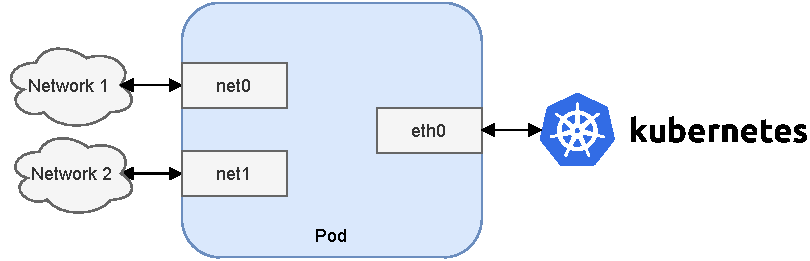
\includegraphics[width=13.5cm]{images/Multus.pdf}
    \caption{Multus enabled pod with two networks}
    \label{fig:Multus}
  \end{center}
\end{figure}

\subsection{SR-IOV}
\label{section:SR-IOV}

I/O throughput is critical to high-performance telco systems. I/O intensive servers may waste CPU cycles waiting for I/O data or spinning on idle cycles, reducing system performance by increasing latency. Single Root I/O Virtualization (SR-IOV) standard allows an I/O device, such as a network interface controller (NIC), to be shared by multiple VMs. The SR-IOV technology is a hardware-based virtualization solution that improves both performance and scalability. \cite{Dong2012}

Traditionally, when a guest accesses the I/O device, VMM needs to intervene in the data processing to share the physical device. The VMM intervention leads to additional I/O overhead for a guest OS. SR-IOV provides hardware enhancements for the Peripheral Component Interconnect Express (PCIe) device, which aims to remove major VMM intervention for performance data movements, such as the packet classification and address translation. An SR-IOV-capable device can create multiple lightweight PCI function entities, known as Virtual Functions (VF). Each VF can be assigned to a VM for direct access but still shares major device resources, achieving both resource sharing and high performance. \cite{Dong2012}

In Kubernetes, Kata Containers supports SR-IOV with a CNI plugin \cite{SR-IOVOpenShift} as visualized in Figure \ref{fig:SR-IOVNode}. Additionally, the Kata runtime detects virtual functions in the container's network namespace to use SR-IOV for network-based devices. In order to enable SR-IOV with Kata, the user needs to install a specific Docker plugin. The created network is based on a physical function device. \cite{SR-IOVKataContainers}

\begin{figure}[ht]
  \begin{center}
    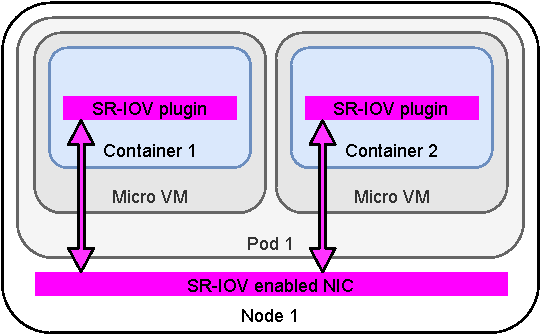
\includegraphics[width=13.5cm]{images/SR-IOVNode.pdf}
    \caption{SR-IOV enabled node with two containers in a single pod}
    \label{fig:SR-IOVNode}
  \end{center}
\end{figure}

In order to set up a host for SR-IOV, the system needs to support Intel Virtualization Technology for Directed I/O (VT-d), and the NIC device needs to support SR-IOV. Also, the host kernel must have Input-Output Memory Management Unit (IOMMU) and Virtual Function I/O (VFIO) support.

\subsection{Hardware acceleration}

Hardware acceleration is the use of hardware specifically crafted to perform functions more efficiently than software running on general-purpose CPUs. The hardware-accelerated process can highly enhance the performance of cloud workloads by increasing throughput and decreasing latency and energy consumption. Hardware acceleration can be used of GPUs for computing, SmartNIC \cite{SmartNICIntel}, or purpose-built application-specific integrated circuit (ASIC) such as System on a Chip (SoC).

The main use of hardware acceleration for edge cloud environment is computing offloading to GPUs, which performs specific workloads faster and frees CPU cycles for other tasks, thus improving throughput. Kata Containers supports passing certain GPU resources from the host into the container using GPU passthrough and GPU mediated passthrough. GPU passthrough, such as Intel GVT-d, allows direct assignment of an entire GPU to a single user, passing the native driver capabilities through the hypervisor without any limitations. Mediated GPU passthrough, such as Intel GVT-g with multiple VMs to one physical GPU, is a full GPU virtualization solution with mediated passthrough. A virtual GPU instance is maintained for each VM, with part of performance-critical resources directly assigned. The ability to run a native graphics driver inside a VM without hypervisor intervention in performance-critical paths achieves a good balance among performance, feature, and sharing capability. \cite{GPUKataContainers}

Plugins such as vAccel \cite{vAccel} offer QEMU and Firecracker VMM support for hardware acceleration for serverless computing. The focus of vAccel is to provide true device sharing in the shared cloud and edge infrastructure with portability and modular design.
		
\section{Logging}

\textcolor{red}{Revisit this chapter}

Kata Containers provides the workload with guest kernel, meanwhile the host uses dedicated kernel, which are not connected. One benefit of the architectural change in comparison to standard container workloads is the availability in case of kernel crashes. This availability is highly beneficial for logging purposes, as the crash of worker container does not wipe all logs at the same time.

\section{Limitations}